\documentclass[11pt, a4paper]{article}\usepackage[]{graphicx}\usepackage[]{xcolor}
% maxwidth is the original width if it is less than linewidth
% otherwise use linewidth (to make sure the graphics do not exceed the margin)
\makeatletter
\def\maxwidth{ %
  \ifdim\Gin@nat@width>\linewidth
    \linewidth
  \else
    \Gin@nat@width
  \fi
}
\makeatother

\definecolor{fgcolor}{rgb}{0.345, 0.345, 0.345}
\newcommand{\hlnum}[1]{\textcolor[rgb]{0.686,0.059,0.569}{#1}}%
\newcommand{\hlsng}[1]{\textcolor[rgb]{0.192,0.494,0.8}{#1}}%
\newcommand{\hlcom}[1]{\textcolor[rgb]{0.678,0.584,0.686}{\textit{#1}}}%
\newcommand{\hlopt}[1]{\textcolor[rgb]{0,0,0}{#1}}%
\newcommand{\hldef}[1]{\textcolor[rgb]{0.345,0.345,0.345}{#1}}%
\newcommand{\hlkwa}[1]{\textcolor[rgb]{0.161,0.373,0.58}{\textbf{#1}}}%
\newcommand{\hlkwb}[1]{\textcolor[rgb]{0.69,0.353,0.396}{#1}}%
\newcommand{\hlkwc}[1]{\textcolor[rgb]{0.333,0.667,0.333}{#1}}%
\newcommand{\hlkwd}[1]{\textcolor[rgb]{0.737,0.353,0.396}{\textbf{#1}}}%
\let\hlipl\hlkwb

\usepackage{framed}
\makeatletter
\newenvironment{kframe}{%
 \def\at@end@of@kframe{}%
 \ifinner\ifhmode%
  \def\at@end@of@kframe{\end{minipage}}%
  \begin{minipage}{\columnwidth}%
 \fi\fi%
 \def\FrameCommand##1{\hskip\@totalleftmargin \hskip-\fboxsep
 \colorbox{shadecolor}{##1}\hskip-\fboxsep
     % There is no \\@totalrightmargin, so:
     \hskip-\linewidth \hskip-\@totalleftmargin \hskip\columnwidth}%
 \MakeFramed {\advance\hsize-\width
   \@totalleftmargin\z@ \linewidth\hsize
   \@setminipage}}%
 {\par\unskip\endMakeFramed%
 \at@end@of@kframe}
\makeatother

\definecolor{shadecolor}{rgb}{.97, .97, .97}
\definecolor{messagecolor}{rgb}{0, 0, 0}
\definecolor{warningcolor}{rgb}{1, 0, 1}
\definecolor{errorcolor}{rgb}{1, 0, 0}
\newenvironment{knitrout}{}{} % an empty environment to be redefined in TeX

\usepackage{alltt}

\usepackage[top=1 in, bottom = 1 in, left = 1 in, right = 1 in ]{geometry}

\usepackage{amsmath, amssymb, amsfonts}
\usepackage{enumerate}

\title{Pie Chart}
\author{Ananda Biswas}
\date{}
\IfFileExists{upquote.sty}{\usepackage{upquote}}{}
\begin{document}

\maketitle

\begin{knitrout}\tiny
\definecolor{shadecolor}{rgb}{0.969, 0.969, 0.969}\color{fgcolor}\begin{kframe}
\begin{alltt}
\hldef{raw_data} \hlkwb{<-} \hlkwd{read.csv}\hldef{(}\hlsng{'https://raw.githubusercontent.com/sakunisgithub/data_sets/refs/heads/master/performance_of_national_parties_in_general_election_2019.csv'}\hldef{)}
\end{alltt}
\end{kframe}
\end{knitrout}

\begin{knitrout}
\definecolor{shadecolor}{rgb}{0.969, 0.969, 0.969}\color{fgcolor}\begin{kframe}
\begin{alltt}
\hlkwd{summary}\hldef{(raw_data)}
\end{alltt}
\begin{verbatim}
##  name_of_the_party  candidates_contested candidates_won  
##  Length:7           Min.   : 34.0        Min.   :  2.00  
##  Class :character   1st Qu.: 55.5        1st Qu.:  4.00  
##  Mode  :character   Median : 69.0        Median : 10.00  
##                     Mean   :207.7        Mean   : 56.71  
##                     3rd Qu.:402.0        3rd Qu.: 37.00  
##                     Max.   :436.0        Max.   :303.00  
##  number_of_votes_secured
##  Min.   :  3576184      
##  1st Qu.:  9622620      
##  Median : 22246501      
##  Mean   : 59795621      
##  3rd Qu.: 72212272      
##  Max.   :229076879
\end{verbatim}
\end{kframe}
\end{knitrout}

\begin{knitrout}
\definecolor{shadecolor}{rgb}{0.969, 0.969, 0.969}\color{fgcolor}\begin{kframe}
\begin{alltt}
\hldef{data.1} \hlkwb{<-} \hldef{raw_data[,}\hlkwd{c}\hldef{(}\hlsng{"name_of_the_party"}\hldef{,} \hlsng{"number_of_votes_secured"}\hldef{)]}
\hlkwd{print}\hldef{(data.1)}
\end{alltt}
\begin{verbatim}
##   name_of_the_party number_of_votes_secured
## 1              AITC                24929330
## 2               BSP                22246501
## 3               BJP               229076879
## 4               CPI                 3576184
## 5            CPI(M)                10744908
## 6               INC               119495214
## 7               NCP                 8500331
\end{verbatim}
\end{kframe}
\end{knitrout}

\begin{knitrout}
\definecolor{shadecolor}{rgb}{0.969, 0.969, 0.969}\color{fgcolor}\begin{kframe}
\begin{alltt}
\hlkwd{summary}\hldef{(data.1)}
\end{alltt}
\begin{verbatim}
##  name_of_the_party  number_of_votes_secured
##  Length:7           Min.   :  3576184      
##  Class :character   1st Qu.:  9622620      
##  Mode  :character   Median : 22246501      
##                     Mean   : 59795621      
##                     3rd Qu.: 72212272      
##                     Max.   :229076879
\end{verbatim}
\end{kframe}
\end{knitrout}


\begin{knitrout}
\definecolor{shadecolor}{rgb}{0.969, 0.969, 0.969}\color{fgcolor}\begin{kframe}
\begin{alltt}
\hldef{slices} \hlkwb{<-} \hlkwd{c}\hldef{(data.1}\hlopt{$}\hldef{number_of_votes_secured)}

\hldef{party_name} \hlkwb{<-} \hlkwd{c}\hldef{(data.1}\hlopt{$}\hldef{name_of_the_party)}

\hldef{party_color} \hlkwb{<-} \hlkwd{c}\hldef{(}\hlsng{"green"}\hldef{,} \hlsng{"grey"}\hldef{,} \hlsng{"orange"}\hldef{,} \hlsng{"red"}\hldef{,} \hlsng{"pink"}\hldef{,} \hlsng{"blue"}\hldef{,} \hlsng{"yellow"}\hldef{)}

\hlkwd{pie}\hldef{(slices,} \hlkwc{main} \hldef{=} \hlsng{"Vote Share of National Parties in GE 2019"}\hldef{,} \hlkwc{col} \hldef{= party_color)}

\hlkwd{legend}\hldef{(}\hlsng{"bottomright"}\hldef{,}
       \hlkwc{legend} \hldef{= data.1}\hlopt{$}\hldef{name_of_the_party,}
       \hlkwc{fill} \hldef{= party_color,}
       \hlkwc{cex} \hldef{=} \hlnum{0.60}\hldef{,}
       \hlkwc{bty} \hldef{=} \hlsng{"n"}\hldef{)}
\end{alltt}
\end{kframe}
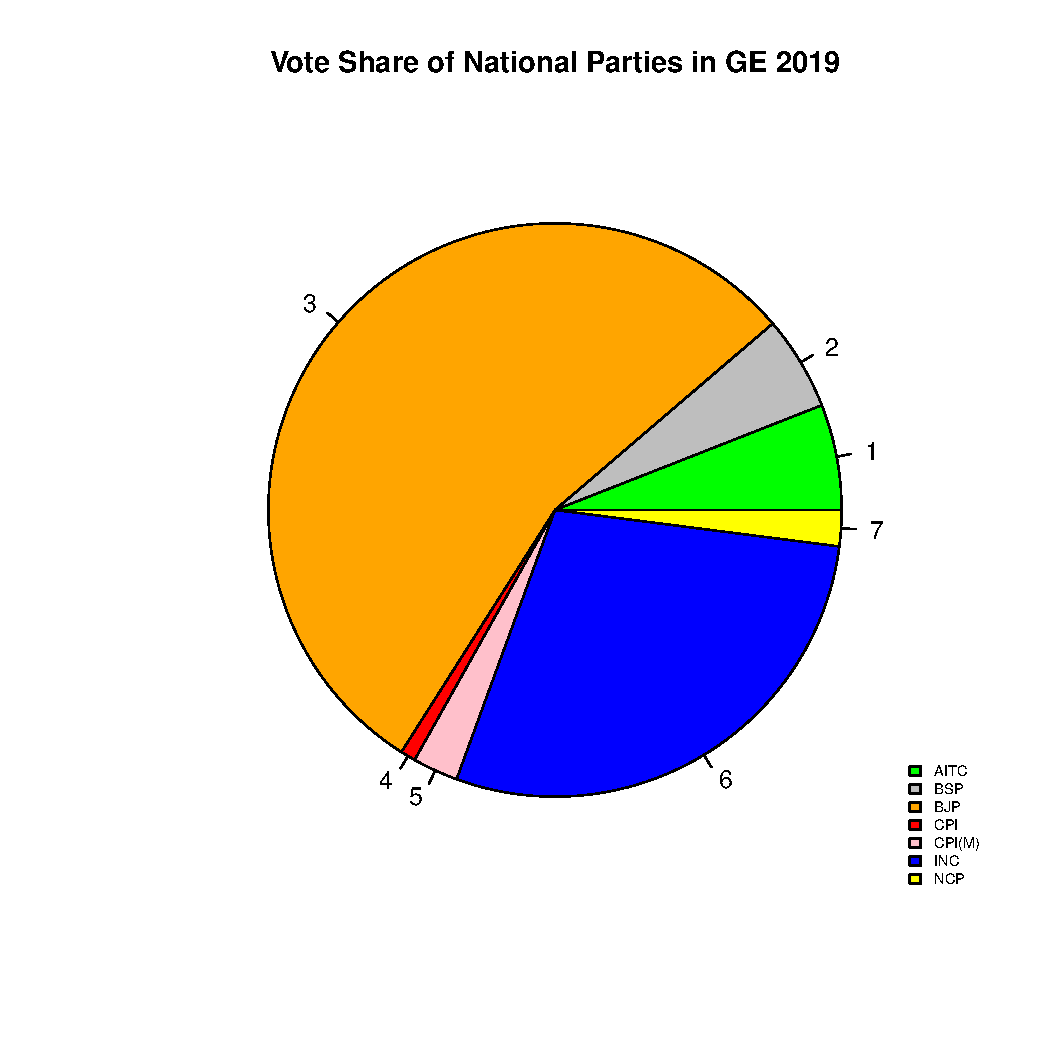
\includegraphics[width=\maxwidth]{figure/unnamed-chunk-5-1} 
\end{knitrout}

$\bullet$ \textit{bty} implies borer-type.

\newpage

\begin{knitrout}
\definecolor{shadecolor}{rgb}{0.969, 0.969, 0.969}\color{fgcolor}\begin{kframe}
\begin{alltt}
\hldef{slice} \hlkwb{<-} \hlkwd{c}\hldef{(data.1}\hlopt{$}\hldef{number_of_votes_secured)}

\hldef{party_names} \hlkwb{<-} \hlkwd{c}\hldef{(}\hlsng{"AITC"}\hldef{,} \hlsng{"BSP"}\hldef{,} \hlsng{"BJP"}\hldef{,} \hlsng{"CPI"}\hldef{,} \hlsng{"CPI(M)"}\hldef{,} \hlsng{"INC"}\hldef{,} \hlsng{"NCP"}\hldef{)}

\hldef{party_colors} \hlkwb{<-} \hlkwd{c}\hldef{(}\hlsng{"green"}\hldef{,} \hlsng{"grey"}\hldef{,} \hlsng{"orange"}\hldef{,} \hlsng{"red"}\hldef{,} \hlsng{"pink"}\hldef{,} \hlsng{"blue"}\hldef{,} \hlsng{"yellow"}\hldef{)}

\hldef{percentage} \hlkwb{<-} \hlkwd{round}\hldef{(slice}\hlopt{/}\hlkwd{sum}\hldef{(slice)}\hlopt{*}\hlnum{100}\hldef{)}

\hldef{lbs} \hlkwb{<-} \hlkwd{paste}\hldef{(party_names, percentage,} \hlsng{"%"}\hldef{,} \hlkwc{sep} \hldef{=} \hlsng{" "}\hldef{)}

\hlkwd{pie}\hldef{(slice,}
    \hlkwc{labels} \hldef{= lbs,}
    \hlkwc{main} \hldef{=} \hlsng{"Vote Share of Different Political Parties in General Election 2019"}\hldef{,}
    \hlkwc{clockwise} \hldef{=} \hlnum{TRUE}\hldef{,} \hlcom{# by default it is set to FALSE}
    \hlkwc{col} \hldef{= party_colors)}
\end{alltt}
\end{kframe}
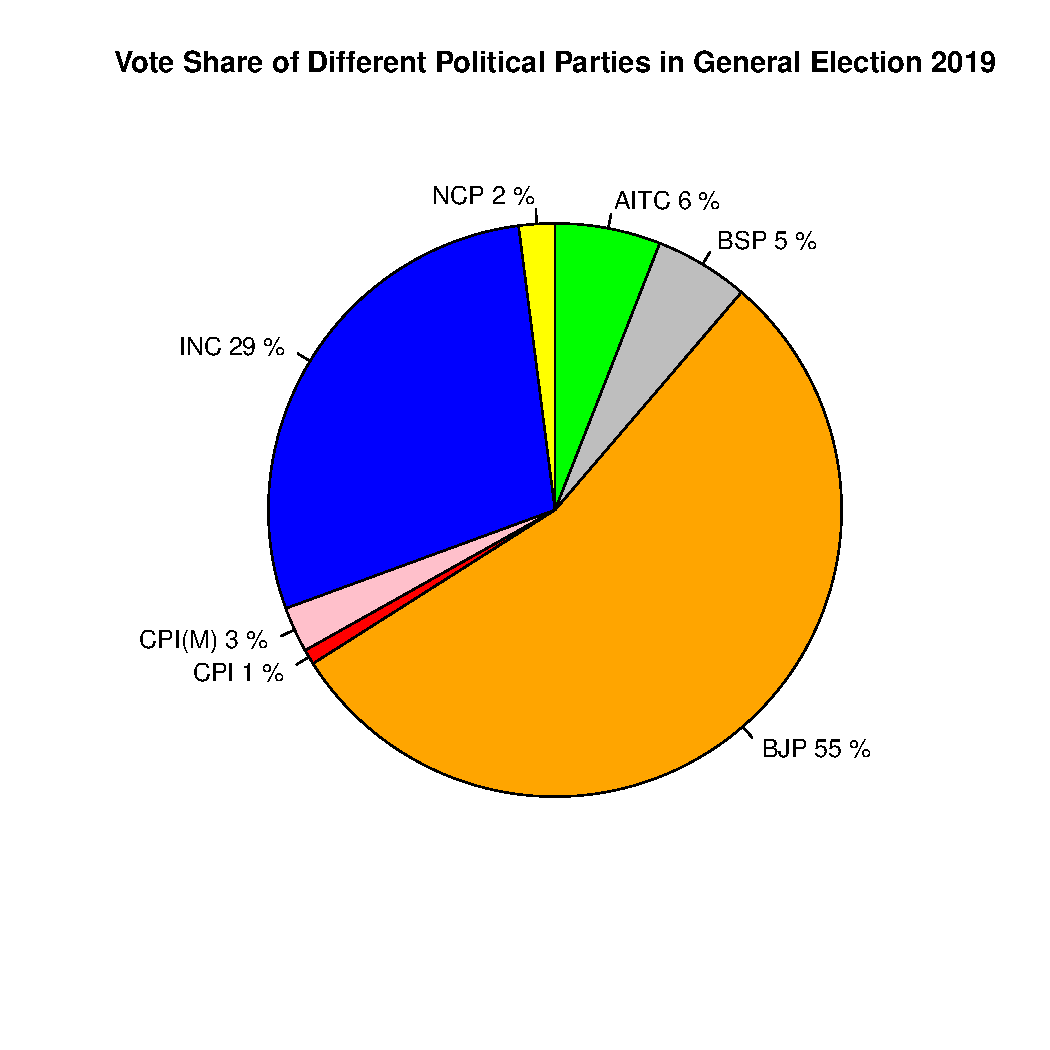
\includegraphics[width=\maxwidth]{figure/unnamed-chunk-6-1} 
\end{knitrout}


\end{document}
